\documentclass{article}

\usepackage{fancyhdr}
\usepackage{extramarks}
\usepackage{amsmath}
\usepackage{amsthm}
\usepackage{amsfonts}
\usepackage{tikz}
\usepackage[plain]{algorithm}
\usepackage{algpseudocode}
\usepackage{dsfont}
\usepackage{subcaption}
\usepackage{lipsum}
\usepackage{ragged2e}

\usetikzlibrary{automata,positioning}

%
% Basic Document Settings
%

\usepackage{graphicx, url}
\graphicspath{figures/}

\topmargin=-0.45in
\evensidemargin=0in
\oddsidemargin=0in
\textwidth=6.5in
\textheight=9.0in
\headsep=0.25in

\linespread{1.1}

\pagestyle{fancy}

% The page Header
\lhead{\hmwkAuthorName}
\chead{\hmwkClassShort}
\rhead{\hmwkTitle}
\lfoot{\lastxmark}
\cfoot{\thepage}

\renewcommand\headrulewidth{0.4pt}
\renewcommand\footrulewidth{0.4pt}

\setlength\parindent{0pt}

%
% Create Problem Sections
%

\newcommand{\enterProblemHeader}[1]{
    \nobreak\extramarks{}{Problem \arabic{#1} continued on next page\ldots}\nobreak{}
    \nobreak\extramarks{Problem \arabic{#1} (continued)}{Problem \arabic{#1} continued on next page\ldots}\nobreak{}
}

\newcommand{\exitProblemHeader}[1]{
    \nobreak\extramarks{Problem \arabic{#1} (continued)}{Problem \arabic{#1} continued on next page\ldots}\nobreak{}
    \stepcounter{#1}
    \nobreak\extramarks{Problem \arabic{#1}}{}\nobreak{}
}

\setcounter{secnumdepth}{0}
\newcounter{partCounter}
\newcounter{homeworkProblemCounter}
\setcounter{homeworkProblemCounter}{1}
\nobreak\extramarks{Problem \arabic{homeworkProblemCounter}}{}\nobreak{}

%
% Homework Problem Environment
%
% This environment takes an optional argument. When given, it will adjust the
% problem counter. This is useful for when the problems given for your
% assignment aren't sequential. See the last 3 problems of this template for an
% example.
%
\newenvironment{homeworkProblem}[1][-1]{
    \ifnum#1>0
        \setcounter{homeworkProblemCounter}{#1}
    \fi
    \section{Problem \arabic{homeworkProblemCounter}}
    \setcounter{partCounter}{1}
    \enterProblemHeader{homeworkProblemCounter}
}{
    \qed
    \exitProblemHeader{homeworkProblemCounter}
}

%
% Homework Details
%   - Title
%   - Due date
%   - Class
%   - Section/Time
%   - Instructor
%   - Author
%

\newcommand{\hmwkTitle}{Homework 1}
\newcommand{\hmwkDueDate}{May, 1}
\newcommand{\hmwkClassShort}{AMATH 563 }
\newcommand{\hmwkClass}{\hmwkClassShort \\ Inferring Structure of Complex Systems}
\newcommand{\hmwkClassTime}{Section A}
\newcommand{\hmwkClassInstructor}{Prof. J. Nathan Kutz}
\newcommand{\hmwkAuthorName}{\textbf{Alexey Sholokhov}}
\newcommand{\hmwkAuthorEmail}{\textit{aksh@uw.edu}}
\newcommand{\hmwkAbstract}{In this assignment we use CINDy -- the model discovery via regression framework. We apply this method to two kinds of data: population time series (the \texttt{Lynx} dataset) and a snippet from a Belousov-Zhabotinsky chemical oscillation video, trying to reveal a Lotka-Volterra model and a Burger equation respectively.}

%
% Title Page
%

\title{
    \vspace{2in}
    \textmd{\textbf{\hmwkClass\\\ \hmwkTitle}}\\
    \normalsize\vspace{0.1in}\small{Due\ on\ \hmwkDueDate\ at 23:59}\\
    \vspace{0.1in}\large{\textit{\hmwkClassInstructor}}
    \vspace{1in}\\
    \justify{\textbf{Abstract: }\hmwkAbstract}
    \vspace{1in}
}


\author{\hmwkAuthorName\\ \hmwkAuthorEmail}
\date{\today}

\renewcommand{\part}[1]{\textbf{\large Part \Alph{partCounter}}\stepcounter{partCounter}\\}

%
% Various Helper Commands
%

% Useful for algorithms
\newcommand{\alg}[1]{\textsc{\bfseries \footnotesize #1}}

% For derivatives
\newcommand{\deriv}[1]{\frac{\mathrm{d}}{\mathrm{d}x} (#1)}

% For partial derivatives
\newcommand{\pderiv}[2]{\frac{\partial}{\partial #1} (#2)}

% Integral dx
\newcommand{\dx}{\mathrm{d}x}

% Alias for the Solution section header
\newcommand{\solution}{\paragraph{Solution} }

% Probability commands: Expectation, Variance, Covariance, Bias
\newcommand{\Var}{\mathrm{Var}}
\newcommand{\Cov}{\mathrm{Cov}}
\newcommand{\Bias}{\mathrm{Bias}}
\newcommand*{\pd}[3][]{\ensuremath{\frac{\partial^{#1} #2}{\partial #3}}}
\newcommand*{\prob}[1]{\ensuremath{\mathbb{P}\left[#1\right]}}
\newcommand*{\ind}[1]{\ensuremath{\mathds{1}_{\left[#1\right]}}}
\newcommand*{\at}[2]{\Big|_{#1}^{#2}}

%
% Different math operators
\DeclareMathOperator{\dom}{Dom}
\DeclareMathOperator{\diag}{Diag}
\DeclareMathOperator{\prox}{prox}
\DeclareMathOperator*{\proj}{proj}
\DeclareMathOperator*{\sign}{sign}
\DeclareMathOperator*{\argmax}{argmax}
\DeclareMathOperator*{\argmin}{argmin}

%% \mathbb symbols
\DeclareMathOperator{\E}{\mathbb{E}}
\DeclareMathOperator{\A}{\mathbb{A}}
\DeclareMathOperator{\R}{\mathbb{R}}
\DeclareMathOperator{\X}{\mathbb{X}}
\DeclareMathOperator{\N}{\mathbb{N}}
\DeclareMathOperator{\Q}{\mathbb{Q}}

%% \mathcal symbols
\DeclareMathOperator{\RR}{\mathcal{R}}
\DeclareMathOperator{\PP}{\mathcal{P}}
\DeclareMathOperator{\NN}{\mathcal{N}}
\DeclareMathOperator{\CC}{\mathcal{C}}
\DeclareMathOperator{\FF}{\mathcal{F}}
\DeclareMathOperator{\YY}{\mathcal{Y}}



\begin{document}

\maketitle
\newpage
\section{Introduction}
Extracting governing equations from data drew a significant attention of a math community over the last decade. Vast availability of data enables computational approach in discovery of natural laws which used to require significant effort for being established theoretically. The most popular tools for model discovery are genetic programming \cite{genetic}, Pareto fronts analysis \cite{pareto}, and regression \cite{kutz}, but other techniques, like equation-free modeling, empirical dynamics modeling, and automated inference of dynamics have been developed as well. 

The natural assumption about the governing equation for macroscale systems is the internal sparsity of models. In particular, a model should contain small number of interpretable terms to be considered as a law, while the big number of terms may evidence overfitting. The regression approach to model discovery utilizes different regularization techniques for sparsity promotion. An example of such technique is the first-norm regularization, which imposes a Laplacian prior to model parameters inducing sparsity of the solution. Total Variation, Elastic Net, and zero-norm regularizers are also in use, yet they make the problem computationally harder. 

In this work we use the SINDy framework \cite{kutz} for model discovery on two types of data: population dynamics time series, which is represented by \texttt{Lynx} dataset, and image data, which is a set of frames from a video of Belousov-Zhabotinsky chemical oscillations. 

\section{Theoretical Background}
\paragraph{Model Discovery via Linear Regression}
Consider a dynamic model 
    \[
        u_t = f(u(x,t)), \quad x \in \R^d, \, t \in \R_+
    \]
    where the governing equation $f(u, t)$ is unknown. Our goal is to discover the equation using a set of data measurements 
    \[
        U = \{(x_i, t_i, u(x_i, t_i)\}_{i=1}^{m}
    \]
    
    We assume that the model $f$ is a sparse linear combination of some terms from a predefined library of candidate functions
    
    \[
        \Theta = \{u, u^2, u^3, u_x, u_y, u_{xx}, u_{yy}, u_{xy} \}
    \]
    
    where all the derivatives are calculated using Finite Difference Method, for instance
    
    \[
        u_t(x_i, t_i) = \frac{u(x_i, t_{i+1}) - u(x_i, t_{i-1})}{2dt}
    \]
    
    It allows us to consider this problem as a linear regression: $A = \Theta(U)$,  $Y = u_t$ so the solution is
    
    \[
        f^*(u) = \Theta\xi^*, \text{ where } \xi^* = \arg \min_{\xi \in \R^{|\Theta|}} \|A\xi - Y\|_2^2 + \frac{\lambda}{2}\|\xi\|_1
    \]
    We use LASSO and Elastic Net -- the first norm regularized linear regression solvers for this problem as we assume the solution $\xi^*$ to be sparse, which prevents overfitting and keeps the model simple.
    
\paragraph{KL divergence} Kullback-Leibler (KL) divergence, is a measure of how one probability distribution is different from a second, reference probability distribution. For two discrete distributions $P(x)$ and $Q(x)$ the KL-divergence is defined as  

    \[
        D_{KL}(P||Q) = \sum_{x \in \mathcal{X}}P(x)\log{\frac{P(x)}{Q(x)}}
    \]
    
    As we don't have an access to a full sample space $\mathcal{X}$, we will use the empirical estimation instead: $\mathcal{X} = U$.
    
\paragraph{AIC} Akaike Information Criteria (AIC) is an estimator of the relative quality of statistical models for a given set of data. Given a collection of models for the data, AIC estimates the quality of each model, relative to each of the other models. 

Suppose that we have a statistical model of some data. Let $k$ be the number of estimated parameters (in our case $k = |\Theta|$), and let $\hat{L}$ be the maximum value of the likelihood function, then the AIC value of the model is the following

\[
    AIC = 2k - 2\log{\hat{L}}
\]

For LASSO we estimate $\hat{L} = \|A\xi^*-Y\|_2^2 + \frac{\lambda}{2}\|\xi^*\|_1$ which is the least square residuals plus penalty. We have to add penalty because it estimates the likelihood of $\xi^*$ having a zero-centered Laplacian distribution: an assumption we implicitly make using LASSO for estimations. 
    
\paragraph{BIC} Bayesian Information Criterion is defined as 
\[
    BIC = k\log(m)-2\log{\hat{L}}
\]
and it is another criterion for model selection: models with lowest BIC are preferred. 

\section{Algorithm Implementation and Development}
This section supplements and clarifies the Jupyter Notebook with the code attached to this homework 
 
\paragraph{Section 1} The first section is devoted to the model discovery for the Lynx-Hare dataset. 
\begin{enumerate}
    \item[1.1)] We put the dataset from the assignment into a \texttt{numpy.array}. We calculate time derivatives and put them into a variable \texttt{Y}. The truncated data is stored in \texttt{X}. We later refer to the Lynx population data as $x_1$ and hare population data as $x_2$. 
    \item[1.2)] We define the library of candidate functions as follows
        \[
            \Theta = \{1, \, x_1,\, x_2,\, x_1^2,\, x_2^2,\,  x_1*x_2,\, x_1^3,\, x_2^3,\, x_1^2x_2,\, x_1x_2^2,\, x_1^4,\, x_2^4,\, \sin{x_1},\, \cos{x_1},\, \sin{x_2},\, \cos{x_2}\}        
        \]
        Note that the Lotka-Volterra equations belong to the linear space of $\Theta$. See \cite{lotka} for references.  
    \item[1.3)] In this section we define two useful functions
        \begin{enumerate}
            \item \texttt{get\_function\_from\_coefs}: this function reconstructs the model for both (Lynx and Hare) time series from the model's coefficients. 
            \item \texttt{kl\_div}: this function computes the KL-divergence of the model. It reconstructs both time series and then returns the distance between the normalized empirical distribution of errors and the normal distribution.
        \end{enumerate}
    
    We use Elastic Net model, which has sparsity promotion capabilities, and, in addition a group sparsity property: groups of correlated features leaves the model together when $\lambda$ increases. This property stabilizes the model's behavior on small datasets, which is the case for this problem.
    
    We try all $\lambda \in [1, 30]$ with step $0.3$, and then plot the results. 
    
    \item[1.4)] This section visualizes the results of the previous experiment. They are illustrated in the figure \ref{fig:lynx_results}
    \item[1.5)] This section illustrates three best models (models with minimal AIC and BIC scores) with their AIC, BIC and KL-divergence scores. They are listed in the table \ref{table:best_fit_models}.
    \item[1.6)] To establish latent variables we calculate an SVD decomposition for the shift matrix of $X$, the number of shifts is 10. We use the \texttt{numpy.svd} function for calculating SVD decomposition.
\end{enumerate}
\paragraph{Section 2} The second section is devoted to the model discovery for a video of Belousov-Zhabotinsky chemical oscillations. 
\begin{enumerate}
\item[1.1)] We use the \texttt{hdf5storage} package for Python to read the Matlab 7.3 file. The data is stored in the variable \texttt{data}. The truncated data (without border pixels) is in the variable \texttt{U}, time derivatives are in the variable \texttt{Y}. No downsampling was used: although being large-scale it still fits to a PC memory and requires reasonable time to process.  
\item[1.2)] As we have an oscillation process, we assume the model to depend on first and second spacial derivatives. We define the library of candidate functions as follows
    \[
        \Theta = \{U,\, U_x,\, U_y,\, U_{xx},\, U_{xy},\, U_{yy}\}
    \]
    
\item[1.3)] We use LASSO as a primary regularized least squares solver for this problem. $\lambda = 10^{-5}$ is fixed and taken to be $\lambda \sim 1/n$ where $n$ is a number of objects. We work with fragments of 300 sequential frames, as it increases the stability of the model and allows us to establish whether coefficients depend on time.
\end{enumerate}
\section{Computational Results}

   \begin{table}
            \centering
            \begin{tabular}{lccc}
                \textbf{Model} & \textbf{$\lambda$} & \textbf{AIC} & \textbf{BIC} \\
                \hline
                $\dot{x} = +0.9348x_1-2.6892x_2+0.0463x_2^2+0.1602\sin(x_1)+0.1251\cos(x_2)$ & 0.01 & 225 & 60 \\
                $\dot{y} =-0.2152x_1-0.8988x_2+0.1599\sin(x_1)-0.0543\cos(x_2)$ & & & \\
                $\dot{x} = +0.4609x_1-0.5500x_2-0.0203x_2^2+0.0261x_1 x_2-0.0764\cos(x_1)+0.0489\cos(x_2)$ & 10 & 205 & 95 \\
                $\dot{y} = -0.0798x_1-0.1338x_2$ & & & \\
                $\dot{x} = +0.4400x_1-0.5123x_2-0.0216x_2^2+0.0263x_1 x_2+0.0274\sin(x_1)-0.0801\sin(x_2)$ & 25 & 190 & 90 \\
                $\dot{y} = -0.0720x_1-0.1182x_2$ 
            \end{tabular}
            \caption{\label{table:best_fit_models}Three best fit models}
        \end{table}
        
    \begin{enumerate}
        \item The model discovery results are represented on the figure \ref{fig:lynx_results}. For each $\lambda \in [1, 30]$ the best fit model is found, its AIC, BIC, and KL-divergence are computed and presented below. We see that for nearly all $\lambda$ the dominant terms in the regression are $x_1$ and $x_2$, which gives us the system 
            \[
                \begin{cases}
                    \dot{x_1} = \alpha x_1 - \beta x_2 \\
                    \dot{x_2} = -\gamma x_1 - \delta x_2
                \end{cases}
            \]
            This is not a Lotka-Volterra model, although the linear terms are correct. 
        \item For all models the KL-divergence is computed and plotted on the middle band of the figure \ref{fig:lynx_results}.
        \item BIC and AIC scores for all the models are presented on the lower part of the figure \ref{fig:lynx_results}. The best models, which correspond to lower values of AIC and BIC, are marked green. Two optimal and one sample best-fit models are listed in the table \ref{table:best_fit_models}. They don't represent data in detail, but they stay finite and approximate the average level: see pictures in the Appendix B for visualization.
        \item The spectre of time-delay embedded system is presented on the figure \ref{fig:lynx_eigen}. We see that the system has many hidden variables, as the eigenvalues decrease gradually. 
    \end{enumerate}
    
    \begin{figure}
        \centering
        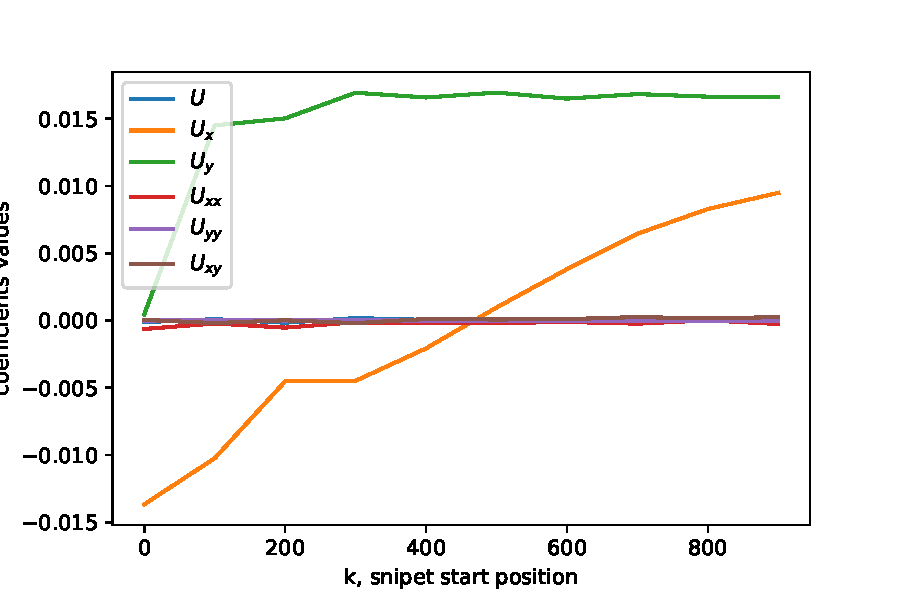
\includegraphics[width=0.8\textwidth]{images/video_coefs.pdf}
        \caption{\label{fig:video_results}Model coefficients depending on the frame start position}
    \end{figure}
    For the second part of the assignment:
    \begin{enumerate}
        \item Best-fit model coefficients for different snippet positions are presented on the picture \ref{fig:video_results}. We see that terms $U_{x}$ and $U_{y}$ remain dominant, although the coefficients change sign over time. The KL-divergence is plotted on the same picture (dotted line) and it gradually decreasing as all the coefficients but two approach zero. Hence the possible model could be
            \[
                U_t = \alpha(t)U_x + \beta(t)U_y
            \]
    \end{enumerate}
    
\begin{figure}[h!]
    \centering
    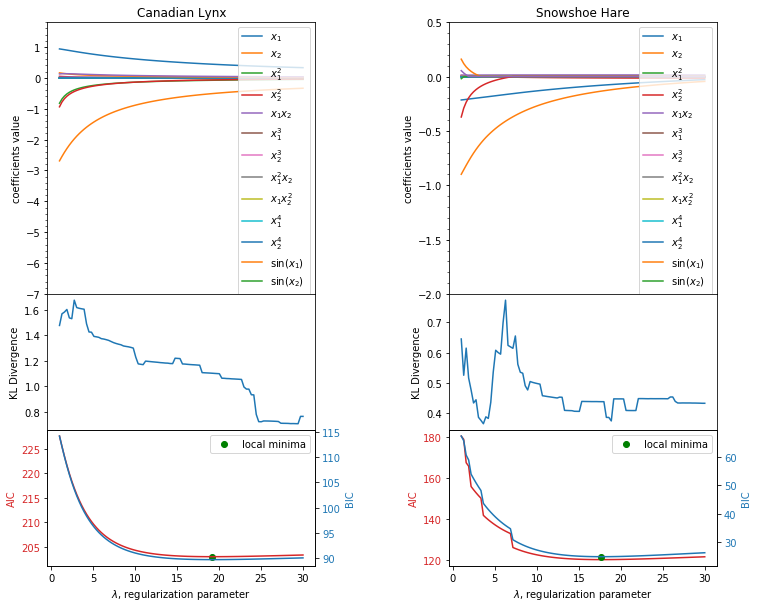
\includegraphics[width=0.9\textwidth]{images/lynx_results.png}
    \caption{\label{fig:lynx_results}
Model discovery illustration}
\end{figure}

\begin{figure}[h!]
    \centering
    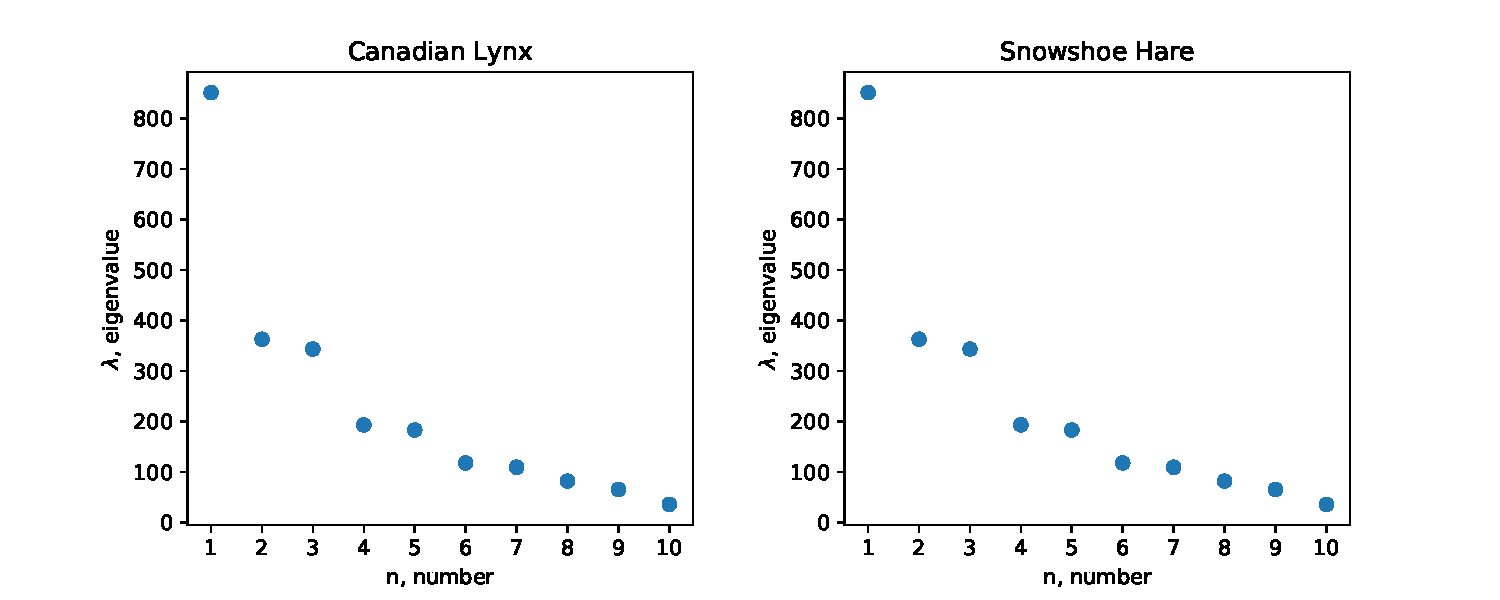
\includegraphics[width=0.85\textwidth]{images/lynx_eigenvalues.pdf}
    \caption{\label{fig:lynx_eigen} Lynx Eigenvalues}    
\end{figure}


\section{Summary and Conclusion}

In this homework we applied a model discovery through regression technique on two datasets. Although the models we got don't exactly match with known models for this kind of systems (Lotka-Volterra model and the Burger equation), they still provide sufficient approximation to the data. 

\begin{thebibliography}{99}

\bibitem{genetic} Bongard, Josh, and Hod Lipson. "Automated reverse engineering of nonlinear dynamical systems." Proceedings of the National Academy of Sciences 104.24 (2007): 9943-9948.
\bibitem{pareto} Schmidt, Michael, and Hod Lipson. "Distilling free-form natural laws from experimental data." science 324.5923 (2009): 81-85.
\bibitem{kutz}Brunton, Steven L., Joshua L. Proctor, and J. Nathan Kutz. "Discovering governing equations from data by sparse identification of nonlinear dynamical systems." Proceedings of the National Academy of Sciences 113.15 (2016): 3932-3937.
\bibitem{lasso}Tibshirani, Robert. "Regression shrinkage and selection via the lasso." Journal of the Royal Statistical Society: Series B (Methodological) 58.1 (1996): 267-288.
\bibitem{lotka}Alfred J. Lotka "Contribution to the Theory of Periodic Reactions"
The Journal of Physical Chemistry 1909 14 (3), 271-274 DOI: 10.1021/j150111a004
\end{thebibliography}
{\_ }
\newpage
\section{Appendix A}
The following non-standard functions were used in this work
\begin{enumerate}
    \item \texttt{hdfs5storage} -- a Python module for working with Matlab 7.3 data, see \url{https://pythonhosted.org/hdf5storage/}
    \item \texttt{IPython.display.Math} -- a wrapper which transforms text input to a Latex picture, see \url{https://ipython.readthedocs.io/en/stable/api/generated/IPython.display.html#IPython.display.Math}
    \item \texttt{IPythin.display.display} -- a function for visual interaction in IPython environment, see \url{https://ipython.readthedocs.io/en/stable/api/generated/IPython.display.html#module-IPython.display}
    \item \texttt{scipy.integrate.solve\_ivp} -- a function which solves initial value problems, see \url{https://docs.scipy.org/doc/scipy/reference/generated/scipy.integrate.solve_ivp.html}
\end{enumerate}


\end{document}
